\chapter{Analisis dan Rancangan Sistem HILS}\label{chapter-3}

Pada Bab \ref{chapter-3} akan dibahas analisis permasalahan pada sistem simulasi yang sudah
ada. Setelah itu, akan dilakukan analisis dan perancangan terhadap solusi yang
akan dibuat pada buku ini.

\section{Deskripsi Umum Proyek \textit{Capstone}}

Tugas akhir yang dikerjakan oleh tim \textit{capstone} bertujuan untuk memenuhi
kebutuhan tim simulasi pada proyek pengembangan trem otonom. Tim simulasi
dibentuk agar pengujian algoritma kendali dan pengumpulan data tidak harus
dilakukan dengan trem yang nyata. Alasannya adalah untuk keamanan, menghemat
biaya, dan menghemat waktu. Pengujian nyata dengan algoritma yang belum siap
dapat menyebabkan orang atau kendaraan lain ditabrak oleh trem. Selain itu,
dengan simulasi para pengembang tidak perlu terjun ke lapangan di Kota Madiun
dan tidak perlu menyewa trem serta rel untuk melakukan pengujian.

Proyek pengembangan trem otonom sendiri dan tim simulasi sudah memasuki tahun
kedua. Akan tetapi, sistem HILS yang ada memiliki banyak masalah, di antaranya
adalah belum adanya skenario simulasi dan kinerja sistem yang buruk. Oleh
karenanya, tim \textit{capstone} perlu memperbarui sistem HILS agar pengujian
HILS dapat dilakukan. Selain itu, tim \textit{capstone} ini juga harus membuat
lingkungan simulasi yang semirip mungkin dengan keadaan di Indonesia serta
membuat beberapa skenario simulasi agar pengujian dapat dilakukan secara
otomatis.

Tugas akhir ini sendiri bertujuan untuk memperbaiki agar sistem HILS dapat
menggunakan sensor virtual dan memiliki dengan kinerja yang baik.  Sistem HILS
sendiri sudah pernah diimplementasi pada tahun pertama proyek, akan tetapi
implementasinya memiliki beberapa keluhan yang akan dibahas pada Subbab
\ref{chapter-3-problems}. Dari keluhan-keluhan tersebut, akan dilakukan analisis
serta rancangan solusi untuk memperbaiki sistem HILS yang ada.

\section{Analisis Masalah Sistem HILS Saat ini}\label{chapter-3-problems}

Pada sistem simulasi saat ini, digunakan tiga komputer:
\begin{enumerate}
	\item komputer SILS: komputer yang menjalankan simulator CARLA dan
	      program-program pembantunya;
	\item komputer AGX: komputer yang akan digunakan trem \textit{production},
	      menjalankan program utama trem otonom yang disebut GRS; dan
	\item komputer RKB: komputer \textit{testbed} untuk komputer  AGX, program
	      yang akan dimuat ke komputer AGX diuji pada komputer ini.
\end{enumerate}

Sistem simulasi yang ada sudah dapat menghubungkan komputer SILS dengan server
komputer RKB/AGX sehingga sistem HILS sudah dapat digunakan. Akan tetapi masih
ada keluhan terkait kinerja sistem HILS, yaitu proses simulasi yang sangat
lambat, menyebabkan simulasi kurang realistis. Jumlah transaksi data per
detik turun dari 4000 transaksi data per detik pada SILS, turun menjadi 100-110
transaksi data per detik ketika menggunakan HILS dan layanan web. Dari ketua tim
simulasi, target kecepatan simulasi yang harus dicapai untuk dianggap cukup
cepat adalah CARLA dapat berjalan stabil dengan minimum 2 FPS (\textit{frames
	per second}).

Padahal kedua komputer pada sistem HILS sudah terhubung pada jaringan lokal
(LAN) yang artinya latensi dan gangguan jaringan akan minimum, jika ada.
Oleh karena itu, kemungkinan \textit{bottleneck} terdapat pada implementasi
mekanisme komunikasi. Implementasi mekanisme komunikasi menggunakan sebuah
layanan web yang arsitekturnya dapat dilihat pada diagram di Gambar
\ref{chapter-2-old-hils}. Proses pada sistem HILS yang sudah ada dapat dilihat
pada diagram sekuens di Gambar \ref{chapter-3-sequence-diagram-old-hils}. Pada
proses pengiriman data, terdapat delapan operasi I/O yang berjalan secara
sinkronis, yaitu
\begin{enumerate}
	\item penulisan CARLA \textit{measurement} ke \textit{file} di SILS,
	\item pembacaan CARLA \textit{measurement} dari \textit{file} di SILS,
	\item pengiriman CARLA \textit{measurement} menggunakan HTTP dari SILS ke
	      layanan web,
	\item penulisan CARLA \textit{measurement} ke basis data pada layanan web,
	\item permintaan HTTP dari AGX/RKB ke layanan web untuk membaca data,
	\item pembacaan CARLA \textit{measurement} dari basis data pada layanan web,
	\item penulisan CARLA \textit{measurement} ke \textit{file} pada AGX/RKB,
	      dan
	\item pembacaan CARLA \textit{measurement} dari \textit{file} pada AGX/RKB.
\end{enumerate}

\begin{figure}[!htbp]
	\centering
	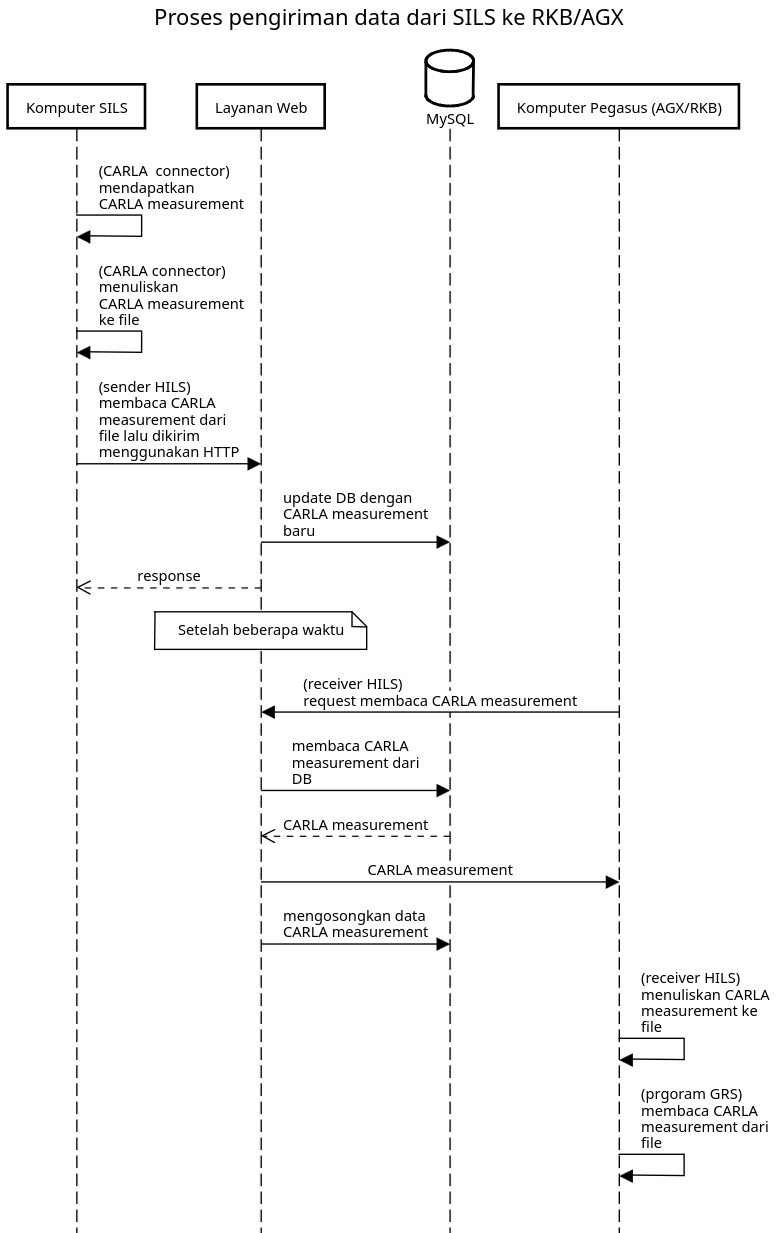
\includegraphics[width=0.9\textwidth]{resources/chapter-3/sequence-diagram-old-hils-process.png}
	\caption{Proses pengiriman data CARLA \textit{measurement} kondisi saat ini}
	\label{chapter-3-sequence-diagram-old-hils}
\end{figure}

Dari diagram sekuens dapat diperkiran \textit{bottleneck} disebabkan
banyaknya operasi I/O sinkronis yang berdampak pada \textit{overhead} operasi
I/O. \textit{Overhead} operasi I/O akan menjadi lebih buruk lagi apabila data
yang dikirimkan berukuran besar, misalnya data sensor kamera. Selain itu, sistem
yang ada juga lebih rumit dari seharusnya. Terdapat perantara berupa layanan web
dan basis data padahal data bisa saja dikirimkan langsung dari komputer SILS ke
komputer AGX/RKB.

Selain masalah kinerja, terdapat keluhan juga karena sistem HILS yang ada belum
menggunakan data sensor. Sistem HILS yang ada masih memanfaatkan CARLA
\textit{measurement}. Data dari CARLA \textit{measurement} mencakup posisi x,
posisi y, kecepatan, dan jarak relatif. Data-data ini dibutuhkan untuk
mendapatkan oleh algoritma kendali, akan tetapi seharusnya didapatkan dari
sensor. Pada sistem HILS saat ini, data \textit{measurement} tersebut didapatkan
dengan memanggil fungsi dari API Python CARLA.

\section{Analisis Solusi}

Dari analisis masalah, didapatkan dua keluhan pada sistem HILS yang ada, yaitu
masalah kinerja dan belum ada dukungan terhadap data sensor. Dari
keluhan-keluhan tersebut, dibutuhkan sebuah solusi yang dapat meningkatkan
kinerja HILS dan dapat menggunakan data sensor. Sensor-sensor yang harus
didukung pada solusi adalah sensor kamera, lidar, dan GNSS. Ketiga sensor harus
dapat digunakan secara bersamaan.

Dari kebutuhan-kebutuhan tersebut, ada dua buah alternatif solusi: melakukan
modifikasi mekanisme komunikasi sistem HILS yang sudah ada atau menulis ulang
mekanisme komunikasi sistem HILS. Dari kedua alternatif, dipilih alternatif
penulisan ulang program HILS. Alasannya adalah karena pada solusi pertama
memiliki kompleksitas yang lebih tinggi karena ada lebih banyak komponen pada
sistem. Selain itu, layanan web pada solusi pertama tidak terintegrasi langsung
pada program utama, baik di komputer SILS maupun komputer AGX/RKB. Layanan web
membutuhkan program bantuan yang berkomunikasi dengan program utama menggunakan
\textit{file}. Hal ini ingin dihindari karena adanya \textit{overhead} I/O.
Selain itu, meskipun layanan web memiliki \textit{coupling} yang rendah dengan
kedua program utama, kohesinya juga rendah. Karena kedua alasan itulah dinilai
alternatif kedua akan lebih mudah untuk dilaksanakan.

Pada proses pembuatan solusi, harus diingat bahwa ada sebuah program utama baru
yang sebelumnya tidak ada, yaitu program yang disebut ScenarioRunner. Program
tersebut merupakan program yang merupakan salah satu tujuan lain dari proyek
\textit{capstone} ini sehingga masih dalam proses pembuatan. Program tersebut
digunakan untuk menjalankan berbagai skenario simulasi dan mengendalikan trem di
CARLA.

Sistem HILS dengan mekanisme komunikasi yang akan ditulis ulang memiliki
kebutuhan-kebutuhan fungsional dan non-fungsional. Kebutuhan fungsional dapat
dilihat pada Tabel \ref{chapter-3-tbl-functional-requirement}. Selain itu,
kebutuhan non-fungsional dapat dilihat pada Tabel
\ref{chapter-3-tbl-non-functional-requirement}.
\begin{table}[!htbp]
	\centering
	\begin{tabular}{|l|l|}
		\hline
		\textbf{Kode} & \textbf{Deskripsi}                                            \\
		\hline
		RF-01         & Program GRS dapat menggunakan data dari sensor kamera virtual \\
		              & CARLA.                                                        \\
		\hline
		RF-02         & Program GRS dapat menggunakan data dari sensor lidar virtual  \\
		              & CARLA.                                                        \\
		\hline
		RF-03         & Program GRS dapat menggunakan data dari sensor GNSS virtual   \\
		              & CARLA.                                                        \\
		\hline
		RF-04         & Program ScenarioRunner dapat menggunakan kendali dari program \\
		              & GRS untuk mengendalikan trem di CARLA.                        \\
		\hline
	\end{tabular}
	\caption{Kebutuhan fungsional sistem simulasi HILS.}
	\label{chapter-3-tbl-functional-requirement}
\end{table}

\begin{table}[!htbp]
	\centering
	\begin{tabular}{|l|l|}
		\hline
		\textbf{Kode} & \textbf{Deskripsi}                                            \\
		\hline
		RN-01         & Sistem simulasi dapat menjalankan simulasi sehingga kecepatan \\
		              & CARLA minimal 2 FPS.                                          \\
		\hline
	\end{tabular}
	\caption{Kebutuhan non-fungsional sistem simulasi HILS.}
	\label{chapter-3-tbl-non-functional-requirement}
\end{table}

Lalu karena dilakukan penulisan ulang mekanisme komunikasi sistem HILS,
protokol/metode komunikasi yang digunakan juga sekalian diubah. Perubahan ini
bertujuan untuk menghilangkan \textit{overhead} yang muncul dari deserialisasi
pesan HTTP. Pesan HTTP mengandung \textit{header} pada pesan \textit{request}
dan respon serta kode status pada pesan respon. Pada HTTP, setiap pesan
\textit{request} yang diterima server harus di-\textit{parse} terlebih dahulu,
lalu pada klien setiap pesan respon harus dibaca dahulu kode statusnya untuk
menentukan \textit{request}-nya berhasil atau tidak \parencite{rfc9110}. Kedua
hal ini tidak digunakan pada sistem HILS. Oleh karena itu, proses deserialisasi
kedua hal tersebut mubazir dan menggunakan \textit{resource} komputer secara
kurang efektif.

Pemilihan mekanisme komunikasi sendiri didasarkan pada studi literatur.
Terdapat dua alternatif untuk mekanisme komunikasi, yaitu ROS 2 dan ZeroMQ.
ROS 2 sendiri adalah sebuah kerangka kerja yang sering digunakan untuk kebutuhan
simulasi robotik. ROS 2 sendiri tidak hanya mengandung ``alat'' komunikasi,
namun memiliki beberapa kakas lain. Sedangkan untuk komunikasinya, ROS 2
fleksibel karena bisa menggunakan pesan ataupun dengan RPC (\textit{remote
	procedure call}). Sedangkan ZeroMQ adalah sebuah pustaka yang dibuat untuk
memberikan peningkatan (\textit{upgrade}) di atas \textit{socket}
tradisional. Komunikasi dengan \textit{socket} dipermudah oleh ZeroMQ karena
abstraksi yang diberikan oleh ZeroMQ. Tidak seperti ROS 2, ZeroMQ menggunakan
pesan untuk komunikasinya. Namun, ada banyak skema komunikasi, misalnya
\textit{publish-subscribe} dan \textit{push-pull}. Beberapa keunggulan dan
kekurangan ROS 2 serta ZeroMQ dapat dilihat pada Tabel
\ref{chapter-3-tbl-ros2-vs-zmq}.

\begin{table}[!htbp]
	\centering
	\begin{tabular}{| r | l | l |}
		\hline
		                    & \textbf{ROS 2}                     & \textbf{ZeroMQ}                                    \\
		\hline
		\textbf{Kelebihan}  & \textit{Tried and tested}          & Sederhana karena hanya                             \\
		                    & untuk kebutuhan aplikasi           & pustaka yang                                       \\
		                    & robotik.                           & mengabstraksikan \textit{socket}.                  \\
		\cline{2-3}
		                    & Adanya dukungan secara             & Dapat menggunakan TCP                              \\
		                    & bawaan untuk format                & secara langsung sebagai                            \\
		                    & data beberapa sensor               & lapisan transpor sehingga         \textit{socket}. \\
		                    & seperti kamera dan                 & mengurangi \textit{overhead}                       \\
		                    & lidar.                             & abstraksi.                                         \\
		\cline{2-3}
		                    & Adanya dukungan untuk              & Memberikan fleksibilitas                           \\
		                    & QoS pesan.                         & dalam menentukan skema                             \\
		                    &                                    & pertukaran pesan.                                  \\
		\hline
		\textbf{Kekurangan} & Adanya \textit{overhead} abstraksi & Pesan dan cara                                     \\
		                    & karena menggunakan DDS             & serialisasi maupun                                 \\
		                    & untuk lapisan transpor.            & deserialisasi pesan harus                          \\
		                    &                                    & didefinisikan dan                                  \\
		                    &                                    & diimplementasikan manual                           \\
		                    &                                    & oleh pengguna ZeroMQ.                              \\
		\cline{2-3}
		                    & Tidak mendukung sistem             & -                                                  \\
		                    & operasi Ubuntu 18.04.              &                                                    \\
		\hline
	\end{tabular}
	\caption{Perbandingan keunggulan dan kelemahan ROS 2 dan ZeroMQ.}
	\label{chapter-3-tbl-ros2-vs-zmq}
\end{table}

Salah satu kekurangan ROS 2 adalah ROS 2 tidak dapat digunakan pada Ubuntu Linux
18.04. Ubuntu 18.04 hanya dapat menggunakan ROS 1. Sayangnya, komputer AGX
menggunakan sistem operasi Ubuntu 18.04 yang dimodifikasi dan RKB juga
menggunakan Ubuntu 18.04. Akibatnya, ROS 2 tidak dapat digunakan pada lingkungan
sistem HILS. Sebenarnya ada jembatan antara ROS 2 dan ROS 1, akan tetapi hal
ini akan menambahkan \textit{overhead} karena perlu adanya komunikasi dengan
jembatan serta perlu konversi pesan antara ROS 2 dan ROS 1.

Oleh karena itu, ZeroMQ dipilih untuk menjadi mekanisme komunikasi sistem HILS
yang baru. Keputusan ini dibuat tidak hanya dengan menimbang kekurangan
inkompatibilitas ROS 2 dengan Ubuntu 18.04, akan tetapi keunggulan ZeroMQ yang
memiliki \textit{overhead} abstraksi lebih kecil juga menjadi poin penting dalam
pemilihan ZeroMQ. Hal ini karena agar kinerja sistem HILS sebaik mungkin,
dampak buruk terhadap kinerja pada sisi komunikasi harus seminimal mungkin.

\section{Rancangan Solusi}

Karena program utama di sisi komputer SILS dan AGX/RKB sudah ada atau sedang
dikerjakan, dipilih solusi dalam bentuk pustaka agar pemuatan fungsionalitas
HILS bisa dilakukan secara modular dan independen dari kedua program utama.
Hal ini menciptakan \textit{coupling} yang rendah antara pustaka dengan kedua
program utama. Selain itu, keuntungan pustaka adalah program GRS jadi dapat
memilih untuk memuat pustaka yang akan dibuat atau tidak pada proses kompilasi
sehingga dapat sedikit menghemat \textit{resource} terutama memori. Pustaka yang
dibuat akan disebut ``hils-connector.''

Pustaka yang akan dibuat ada dua, yaitu pustaka C++11 untuk program GRS di
komputer AGX/RKB dan pustaka Python 3 untuk \textit{agent} program
ScenarioRunner. Pustaka Python akan disebut ``\textit{producer}'' karena
memproduksi data sensor. Pustaka C++ akan disebut ``\textit{consumer}'' karena
mengonsumsi data sensor. Selain data sensor, juga akan ada data berupa
kontrol/perintah dengan format sebuah \texttt{int} yang dikirim dari
\textit{consumer} ke \textit{producer} setelah data sensor berhasil diproses.

Lalu untuk fitur pustaka itu sendiri, pustaka akan langsung berkomunikasi satu
sama lain tanpa menggunakan perantara. Hal ini membuat solusi lebih sederhana
dan mengurangi \textit{overhead} untuk berkomunikasi dengan perantara. Pustaka
juga akan menyediakan API untuk mengirimkan data dan menerima data. Untuk
mendukung berbagai jenis sensor, pustaka juga akan memiliki fitur
\textit{parsing}, serialisasi, dan deserialisasi untuk sensor GNSS, kamera, dan
lidar.

API yang disediakan oleh pustaka ``producer'' akan langsung mengonsumsi data
sensor dari CARLA sehingga pengguna pustaka tidak perlu melakukan modifikasi
apapun pada data sensor CARLA. Begitu juga pada pustaka ``consumer''. Balikan
API akan disesuikan sehingga pengguna pustaka dapat langsung menggunakan data
sensor dan langsung ``memasukkannya'' ke sensor virtual NVIDIA DriveWorks.

Lalu, untuk mengurangi berbagai \textit{overhead} tambahan yang dapat muncul
karena operasi pada jaringan, dipilih mekanisme komunikasi menggunakan ZeroMQ.
ZeroMQ adalah \textit{message queue} sehingga cocok digunakan untuk operasi
asinkron yang sesuai dengan pengiriman data sensor dari CARLA. Lalu, ZeroMQ juga
sangat dekat dengan TCP, tapi tanpa kompleksitas \textit{raw} TCP. Hal tersebut
dikarenakan salah satu tujuan utama ZeroMQ adalah mengurangi latensi hinga
sesedikit mungkin dan memaksimalkan \textit{throughput}. ZeroMQ juga tidak
memiliki \textit{broker}, hal ini sesuai dengan keinginan menghilangi perantara
sehingga \textit{producer} dan \textit{consumer} dapat langsung berkomunikasi
satu sama lain.

Dari solusi pustaka yang ditawarkan, dapat dibentuk sebuah arsitektur sistem
HILS. Arsitektur ini dapat dilihat pada diagram \textit{deployment} di Gambar
\ref{chapter-3-new-architecture}. Lalu, gambaran kasar proses pada sistem
simulasi untuk satu \textit{step} simulasi dapat dilihat pada diagram
sekuens di Gambar \ref{chapter-3-new-sequence}. Perlu dicatat bahwa HILS
\textit{agent} adalah \textit{agent} yang digunakan pada program
ScenarioRunner.

\begin{figure}[!htbp]
	\centering
	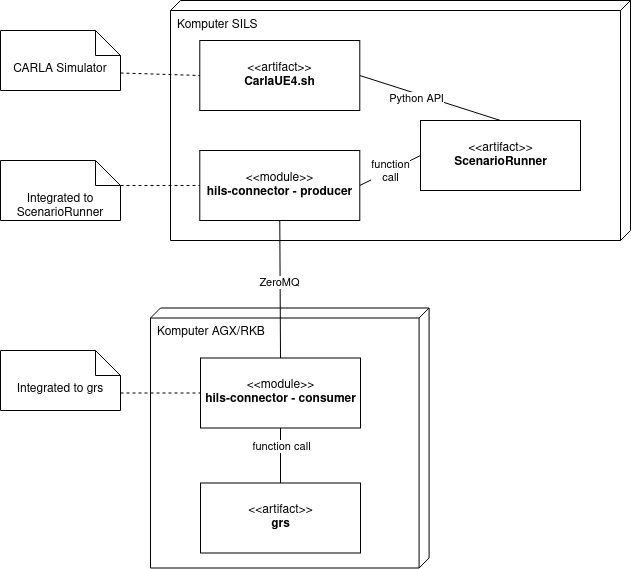
\includegraphics[width=1.0\textwidth]{resources/chapter-3/deployment-diagram-new-hils.png}
	\caption{Arsitektur Sistem HILS Baru}
	\label{chapter-3-new-architecture}
\end{figure}

\begin{figure}[!htbp]
	\centering
	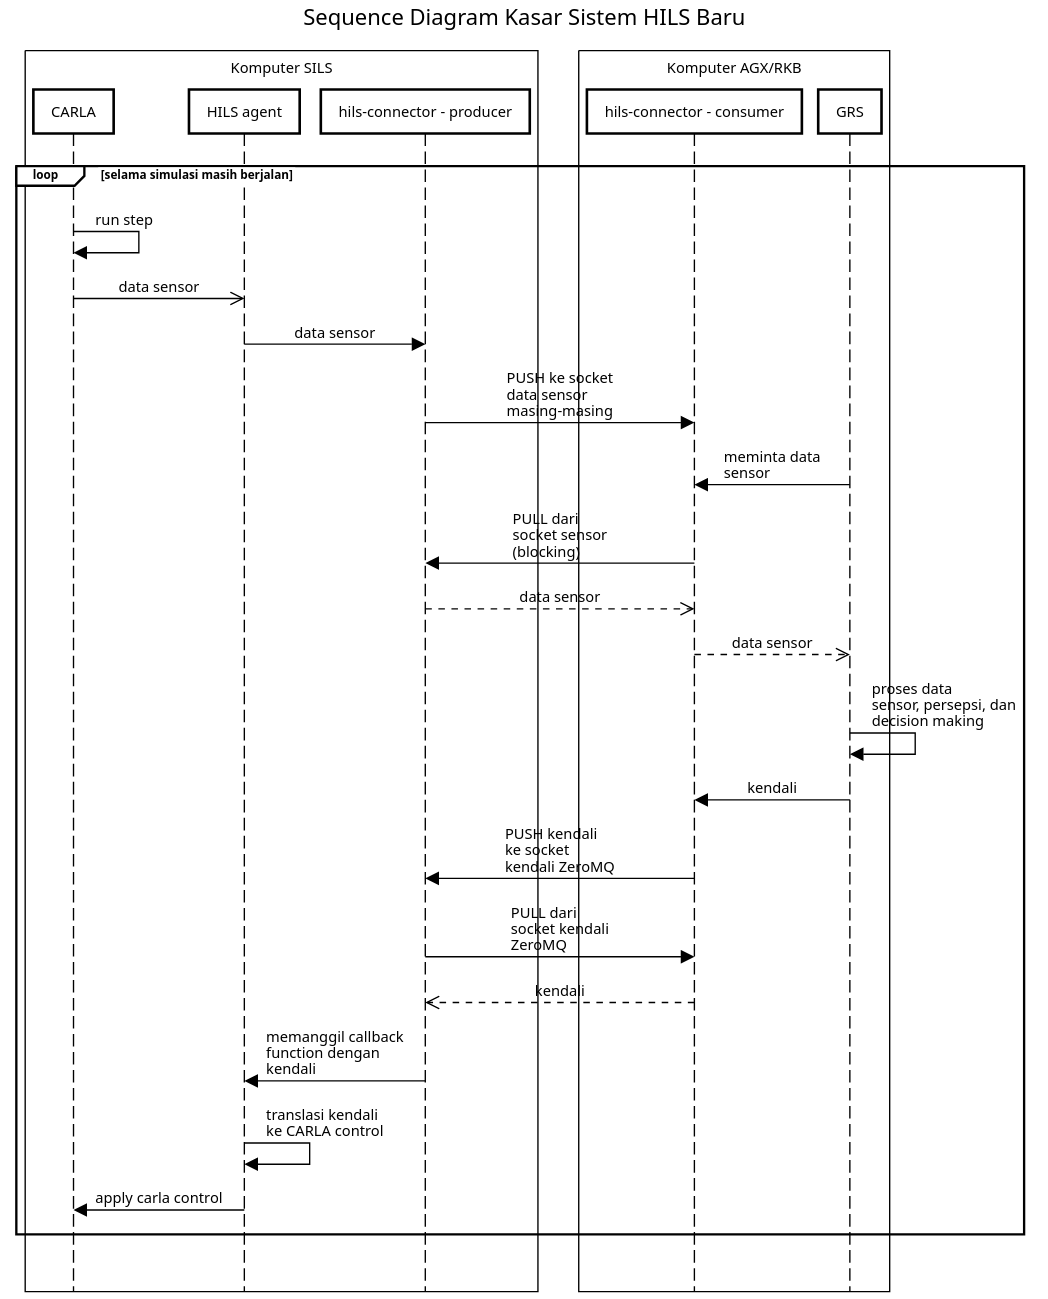
\includegraphics[width=1.0\textwidth]{resources/chapter-3/sequence-diagram-new-hils-kasar.png}
	\caption{Gambaran kasar proses satu \textit{step} simulasi}
	\label{chapter-3-new-sequence}
\end{figure}
